\documentclass{beamer-control}
\usepackage{beamer-control-singlefile}
\INCLUDEONLY{Modeling Concepts}
\begin{document}
\CONCEPT{Modeling Concepts}

\begin{SUMMARY}
\begin{itemize}
\item Systems, models
\item Variables, states, `state space'
\item Example of nonlinear model output
\item Example of linear time-invariant model output
\item Standard control equation
\end{itemize}
\vfill References:
\begin{itemize}
\item \astrom{§3.1}
\end{itemize}
\end{SUMMARY}


\begin{frame}{Systems and models}

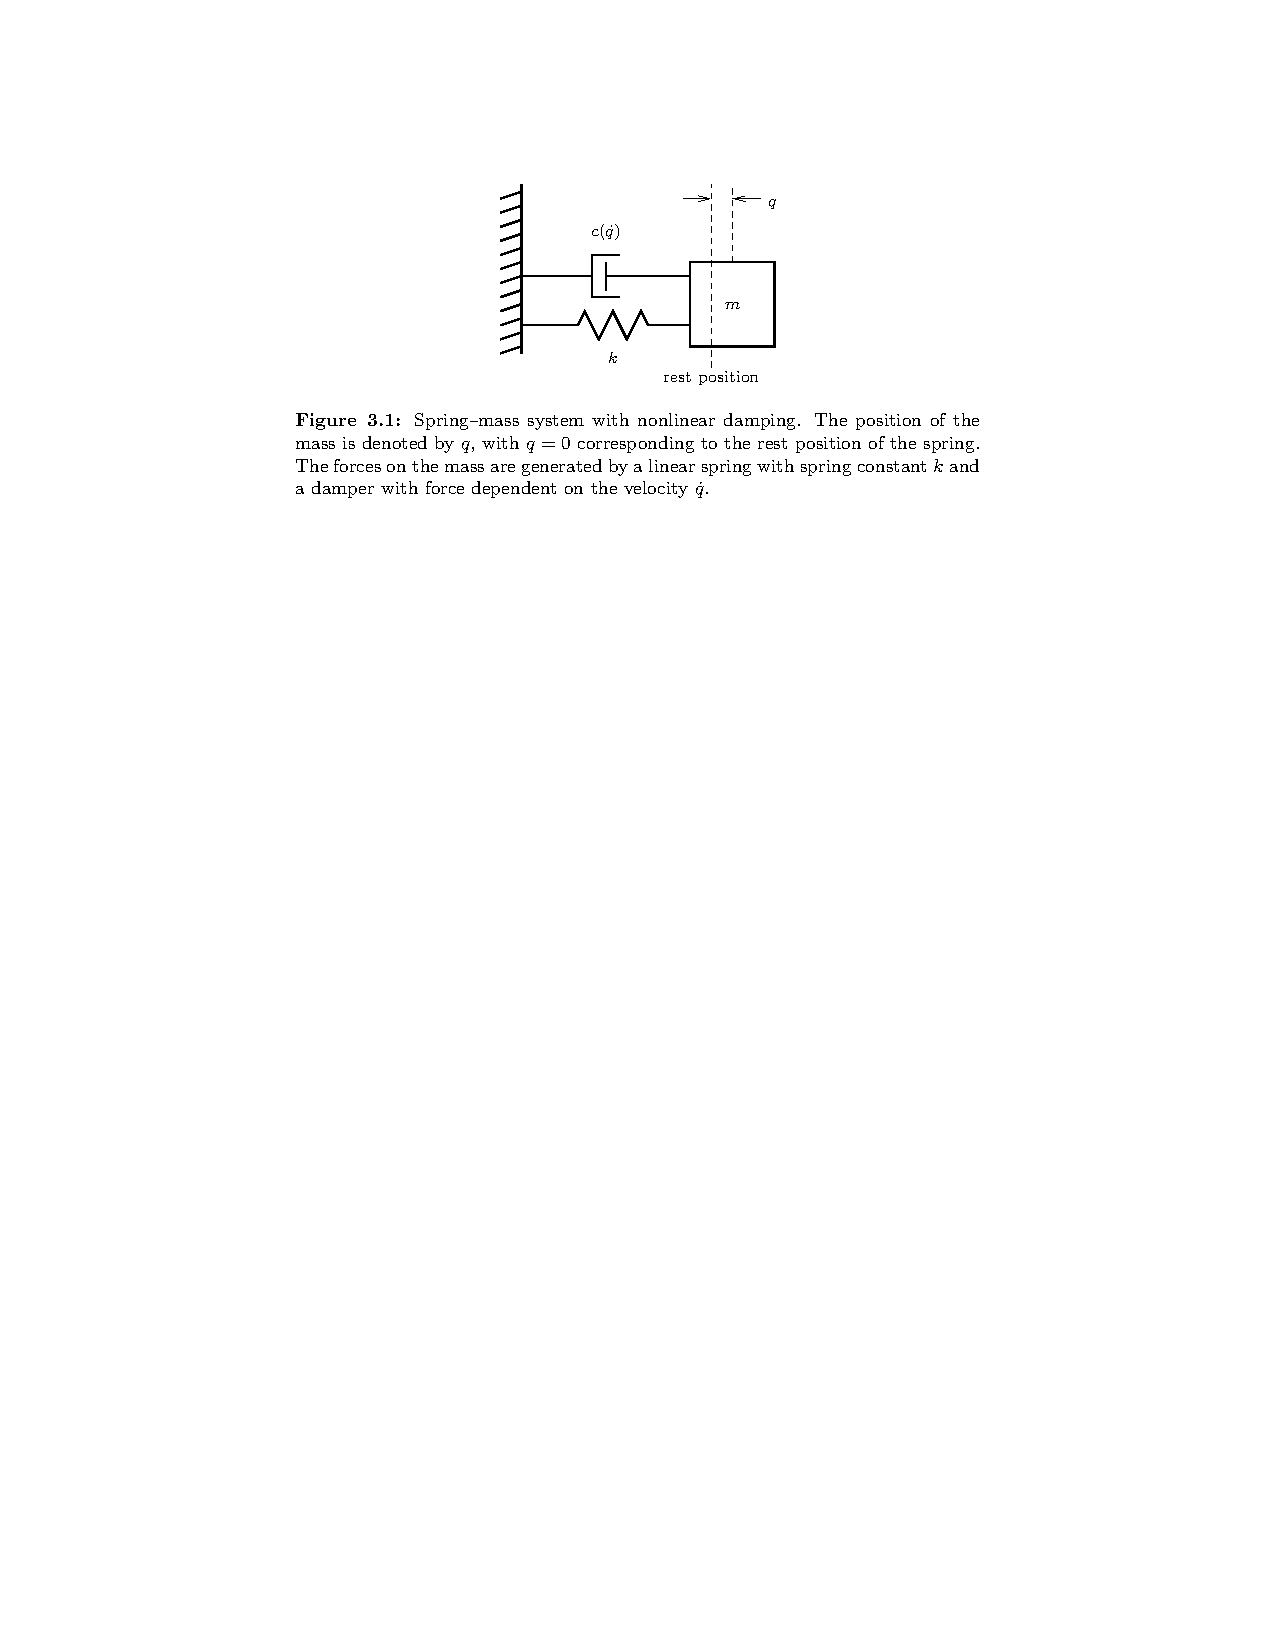
\includegraphics[width=\linewidth]{figure3.1}

\end{frame}

\begin{frame}
\frametitle{State model --- mass-spring-damper with nonlinear damping}

\vspace*{-5mm}
\begin{align}
m \ddot q + c(\dot q) + kq &= 0 & x &= \Matr{q\\ \dot q}
\end{align}

\centering
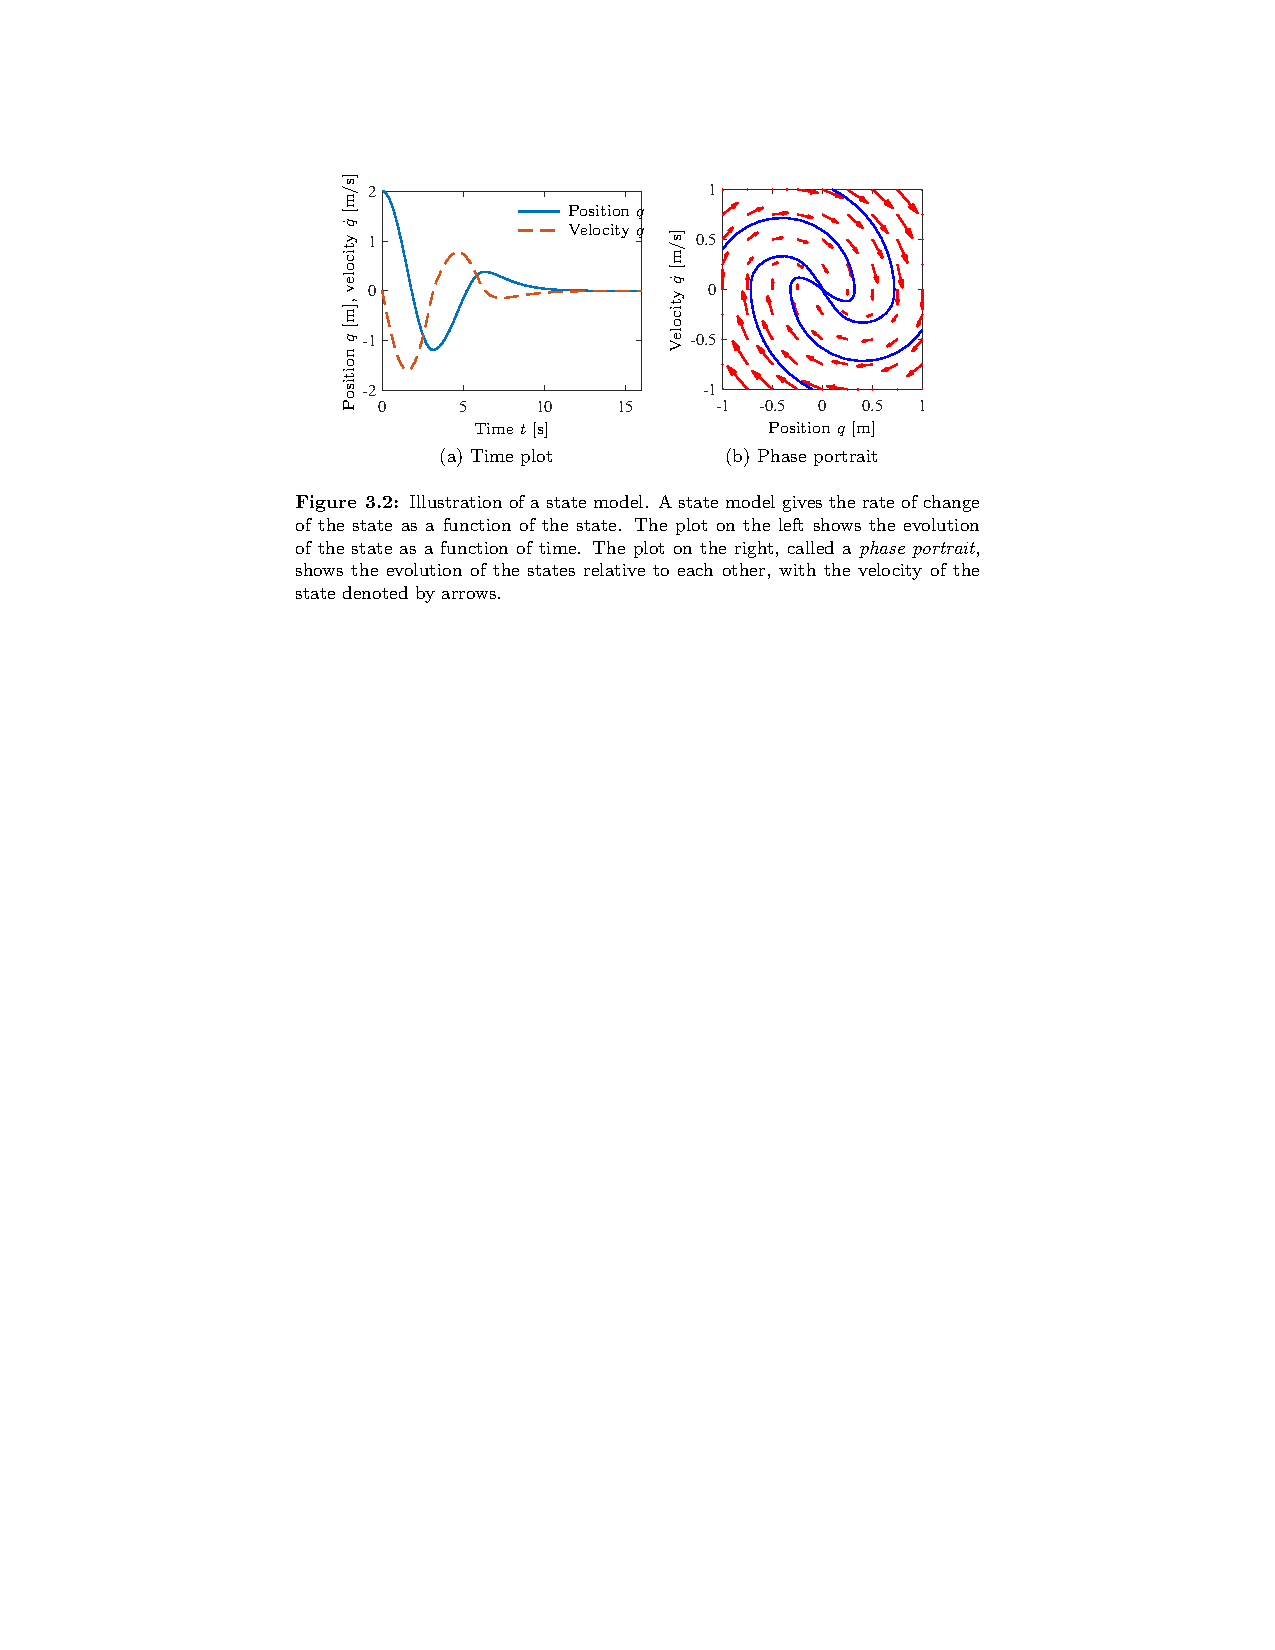
\includegraphics[width=0.9\linewidth]{figure3.2}

\end{frame}

\begin{frame}
\frametitle{Input-output models}
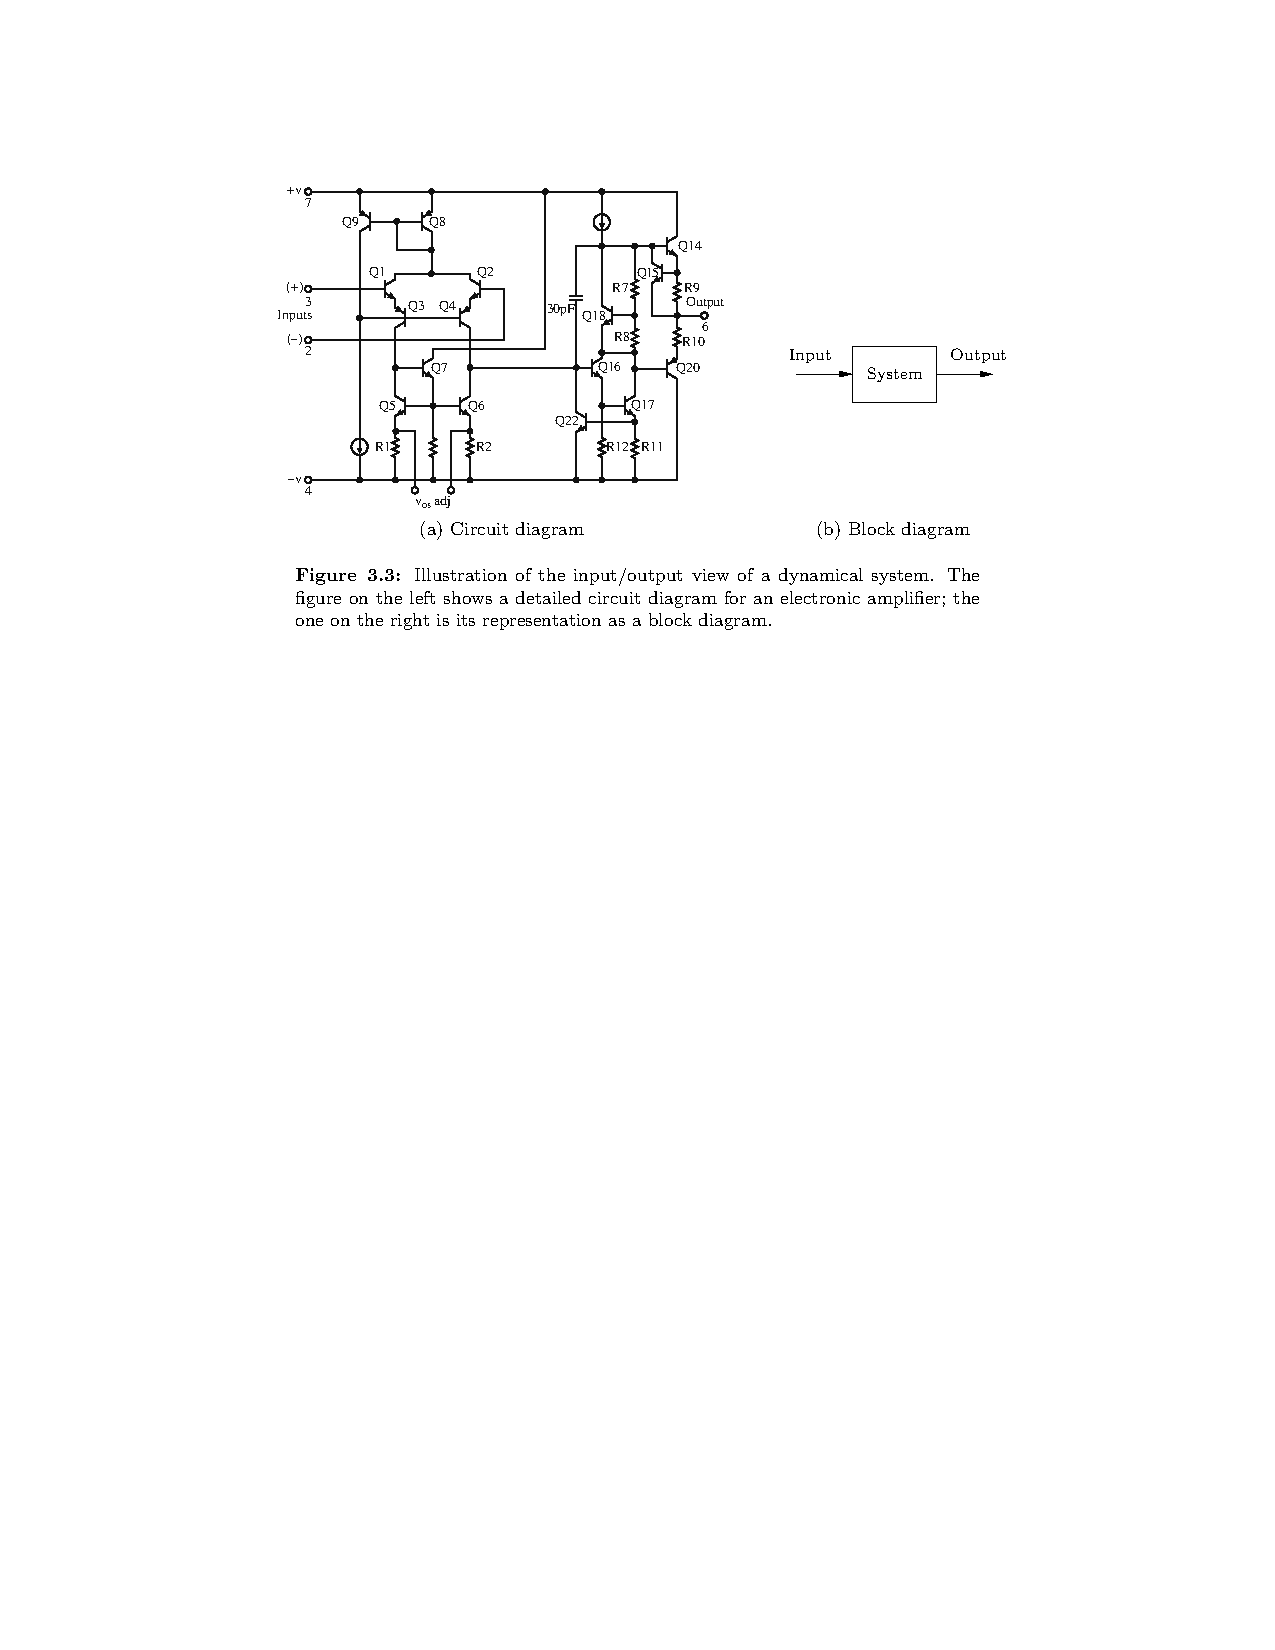
\includegraphics[width=\linewidth]{figure3.3}
\end{frame}

\begin{frame}
\frametitle{Linear time-invariant models}
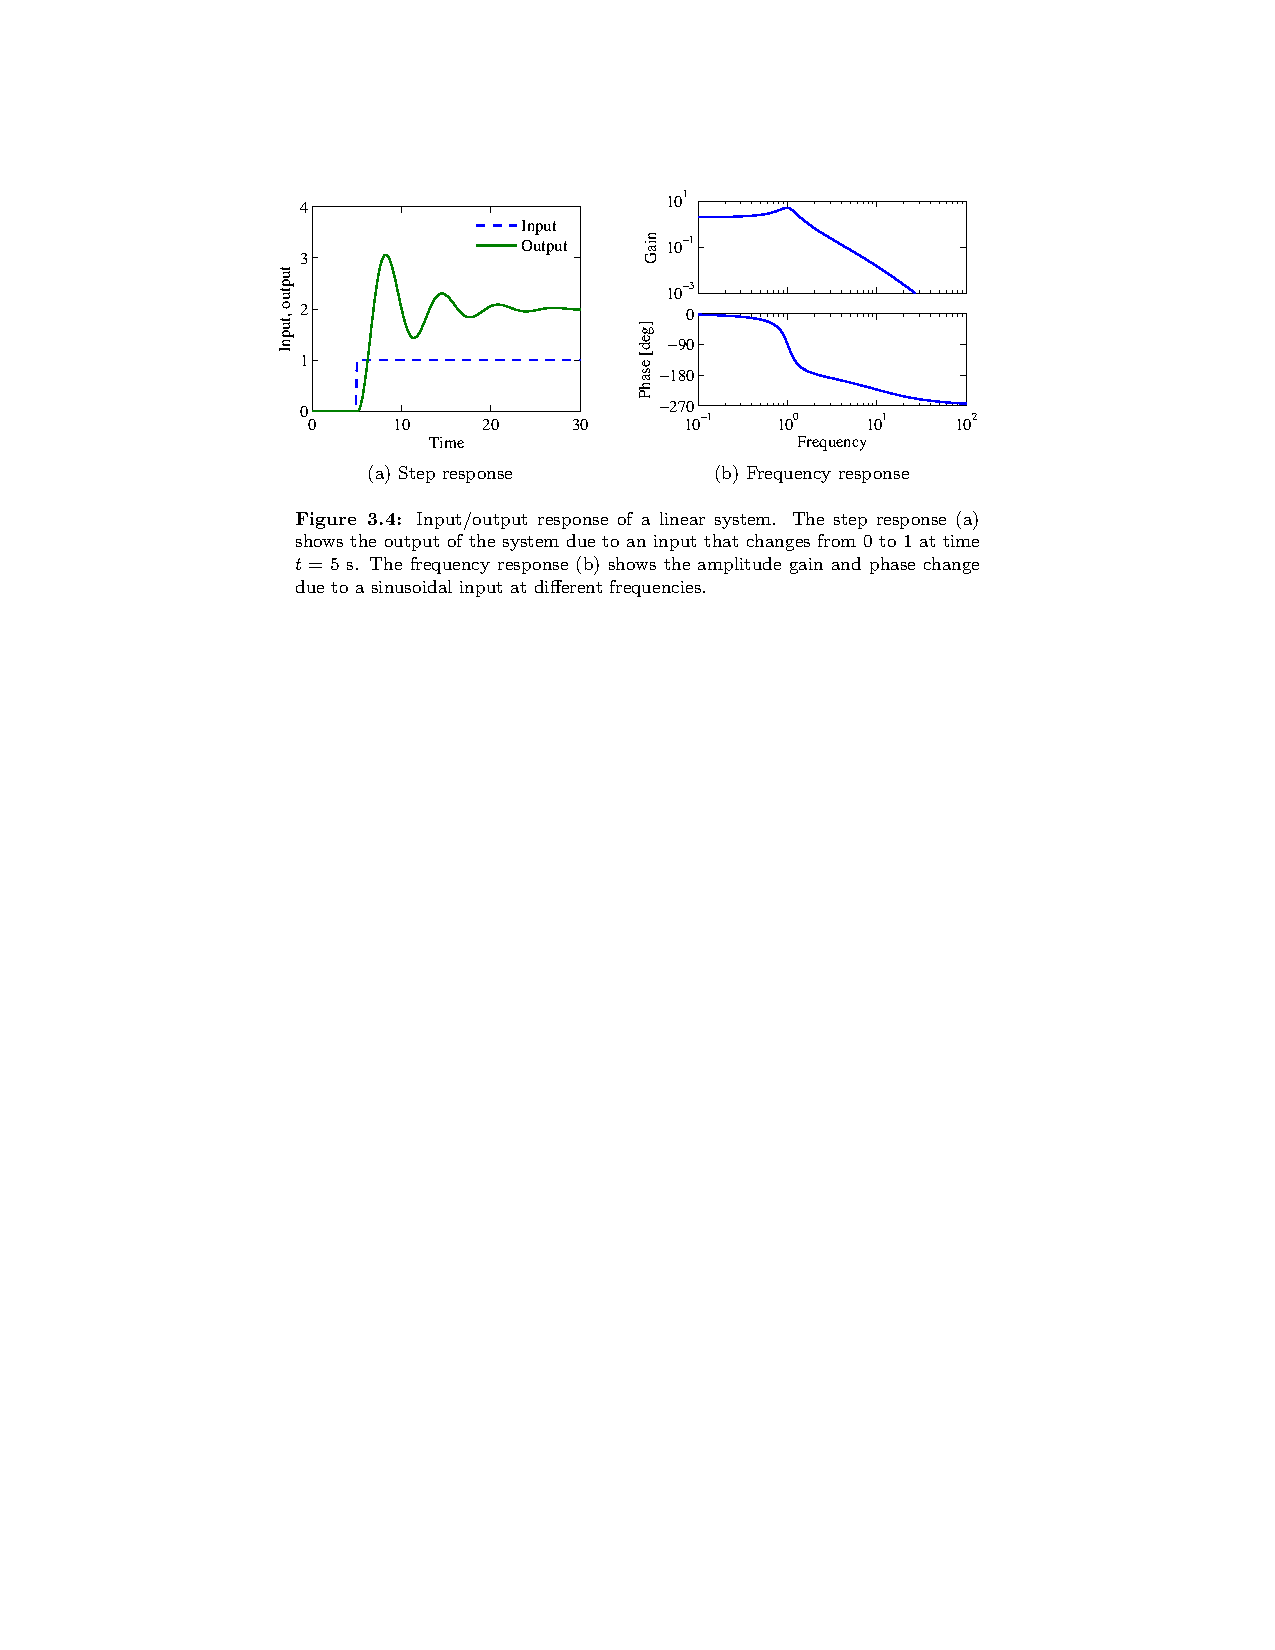
\includegraphics[width=\linewidth]{figure3.4}
\end{frame}

\begin{frame}
\frametitle{Standard nonlinear control equation}
\begin{align}
\Deriv{x}{t} &= f(x,u) & y &= h(x,u)
\end{align}
Recall nonlinear spring example with $x = [q\quad \dot q]\Tr$:
\begin{align}
\Deriv{x}{t} &= \begin{bmatrix}\dot q\\\ddot q\end{bmatrix} = \begin{bmatrix}\dot q\\- c(\dot q)/m - kq/m\end{bmatrix}
\end{align}
If we measure displacement $q$:
\begin{align}
y = h(x,u) &= q
\end{align}
Use these equations to simulate, simplify, analyse\dots

\end{frame}



\SUMMARYFRAME
\FINALE

\end{document}
